% !TEX encoding = UTF-8 Unicode
\chapter{Donn\'ees}
\label{chap2}
%\minitoc
%Dans cette chapitre je vais pr\'esenter sur les s\'eries temporelle, les donn\'ees \'epidemiologies et environnementaux. Puis je présente les étapes de prétraitement des donn\'ees
\section{Les séries temporelles}
\subsection {Définition}
Une série temporelle est une série de points de données indexées (ou répertoriés ou représentés graphiquement) dans l'ordre chronologique. Plus précisément,  une série temporelle est une séquence prise à des points successifs espacés régulièrement dans le temps ou on peut rappelé une séquence de données en temps discret. Les séries temporelles sont utilisées dans les statistiques, le traitement du signal, la reconnaissance des formes, l'économétrie, la finance mathématique, la prévision météorologique, l'électroencéphalographie, l'ingénierie de contrôle, l'astronomie, l'ingénierie des communications et dans tous les domaines de la science appliquée. 

Une série chronologique normale comprend 4 parties:
\begin{itemize} 
\item[$\bullet$] Niveau : La valeur de référence pour la série s'il agissait d'une ligne droite.
\item[$\bullet$] Tendance : Le comportement croissant ou décroissant optionnel et souvent linéaire de la série dans le temps.
\item[$\bullet$] Saisonnalité : Les motifs ou les cycles répétitifs facultatifs de comportement dans le temps.
\item[$\bullet$] Bruit : La variabilité optionnelle des observations qui ne peut être expliquée par le modèle.
\end{itemize} 
Toutes les séries temporelles ont un niveau, la plupart ont du bruit, la tendance et saisonnalité sont optionnelles. 

\subsection{Analyse des séries temporelles}
L'analyse de séries temporelles comprend des méthodes d'analyse de données de séries temporelles afin d'extraire des statistiques significatives et d'autres caractéristiques des données. Il existe de nombreuse des applications de l'analyse des séries temporelles et ils sont largement utilisés dans les différences domaines de recherche.

L'application qui est utilisé plus souvent est la prédiction de série temporelle. Il utilise un modèle pour prédire des valeurs futures basées sur des valeurs précédemment observées. Dans le traitement statistique classique sur des données de séries temporelles, la prédiction sur le futur s'appelle l'extrapolation. Une distinction importante dans la prédiction est que l'avenir est complètement indisponible et doit seulement être estimé à partir de ce qui est déjà arrivé. La compétence d'un modèle de prévision de série temporelle est déterminée par sa performance à prédire l'avenir. Cela se fait souvent au détriment de pouvoir expliquer pourquoi une prédiction spécifique a été faite, des intervalles de confiance et encore mieux comprendre les causes sous-jacentes du problème.

Une autre application est l'analyse de régression qui est souvent utilisée de manière à tester les théories selon lesquelles les valeurs actuelles d'une ou plusieurs séries temporelles indépendantes affectent la valeur courante d'une autre série temporelle, ce type d'analyse de séries temporelles se concentre sur la comparaison des valeurs d'une série temporelle unique ou de séries temporelle dépendantes multiples à différents moments.

\section{Les donn\'ees de la dengue}
Nous avons utilisé des données mensuelles de surveillance de la dengue provenant des provinces de huit pays couvrant une zone géographique de 3 500 kilomètres d'est en ouest sur 2 500 kilomètres du nord au sud et qui comptaient une population combinée de 320 millions en 2010. Des données mensuelles sur la surveillance de la dengue et les données démographiques et climatiques correspondantes au niveau provincial étaient disponibles pour 273 provinces en Thaïlande, au Cambodge, au Laos, au Vietnam, en Malaisie, en Indonésie, aux Philippines et à Taïwan. Les nombres des cas de dengue mensuels  ont été calculés de 1993 à 2010 pour les provinces de Thaïlande, de Malaisie et de Singapour, de 1994 pour les Philippines et le Vietnam et de 1998 pour les autres pays\cite{van2015}. Nous avons calculé les taux d'infection en divisant le nombre des cas de dengue de chaque mois par le nombre de population typique pour chaque provinces.  Les données des zones administratives globales (GADM, www.gadm.org) des pays en Sud-Est d'Asie ont été utilisées pour les visualisation géographiquement. La visualisation des taux d'infection sont présenté sous forme une vidéo. 

La figure 2.1 représente quelques images export de la vidéo qui exprime des importants situations de la taux d'infection durant la période 1994 - 2010. Le taux d'infection des provinces est représentées de moins au plus d'infection en degré croissant de couleur rouge. C'est à dire les provinces qui ont eu moins infection était en couleur jaune, tandis que les provinces avec le taux d'infection élevé sont eu le couleur rouge. Les provinces manquant les données sont représenté en couleur noir. Les deux ligne rouge horizontal représente le zone tropical. Le premier sommet de l'épidémie de la dengue en Juillet 1994 est présenté en figure 2(a). On peut voir que dans le durée à partir Janvier 1994 jusqu'au Décembre 1997, les taux d'infections viennent des pays comme Thaïlande, Vietnam, Malaisie, Philippines et quelques province de Taïwan. Pendant cette période, le sommet du taux d'infection de chaque années tombait souvent au mois Juillet. La figure 2(b) montre le moment au Août 1998 - la sommet le plus élevé durant toutes la période après l'ajouté les données du Laos et du Cambodge à partir du Janvier 1998. Au début du Janvier 1999, le donné du dernière pays, l'Indonésie, se joindre au modèle et se représente dans la figure 2(c). Ensuite, les deux sommet typique du taux d'infection sont présenté aux figures 2(d) - Juillet 2001 et 2(e) - Mars 2004. Les données de l'Indonésie sont terminé en Avril 2005 et se représente dans la figure 2(f). Les deux dernière sommet les plus élevé apparait en Juillet 2007(figure 2(g)) et Août 2010 (figure 2(h)). On peut voir que les sommets d'infection des années sont toujours tombée sur les mois Juillet et Août.  Les taux d'infection dans des pays tels que le Vietnam, la Thaïlande, la Malaisie et les Philippines sont souvent plus élevés que dans d'autres pays. Cela peut être affecté par les conditions météorologiques de la mousson de la région. 
\begin{center}
\begin{minipage}{0.5\textwidth}
\captionof*{figure}{(a)Taux d'infection en Juillet 1994  }
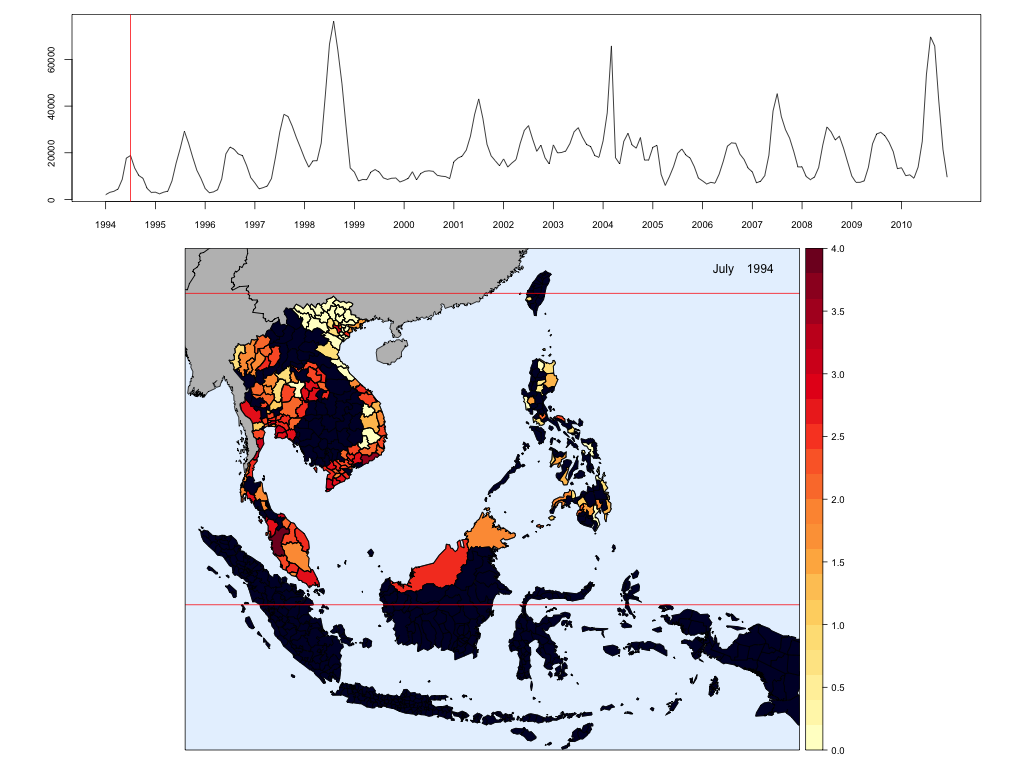
\includegraphics[width=\linewidth]{../figures/chap2/Test7.png}
\label{fig2a}
\end{minipage}\hfill
\begin{minipage}{0.5\textwidth}
\captionof*{figure}{(b)Taux d'infection en Août 1998}   
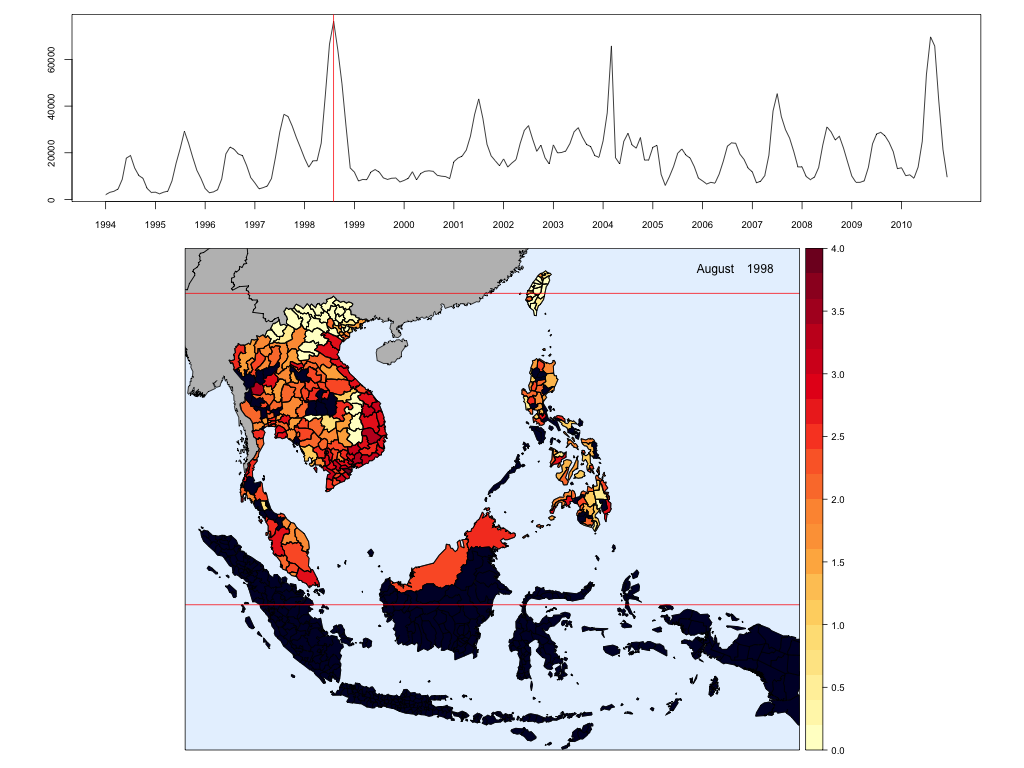
\includegraphics[width=\linewidth]{../figures/chap2/Test56.png} 
\label{fig2b}
\end{minipage}
\begin{minipage}{0.5\textwidth}
\captionof*{figure}{(c)Taux d'infection en Janvier 1999  }
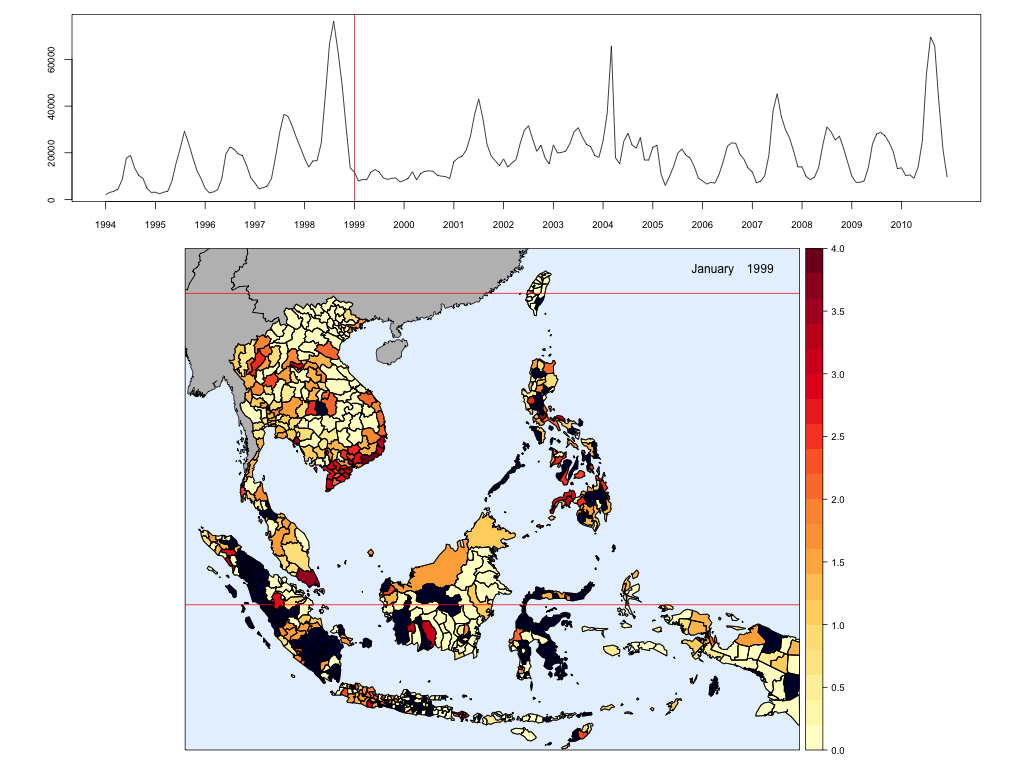
\includegraphics[width=\linewidth]{../figures/chap2/Test61.png}
\label{fig2c}
\end{minipage}\hfill
\begin{minipage}{0.5\textwidth}
\captionof*{figure}{(d)Taux d'infection en Juillet 2001}   
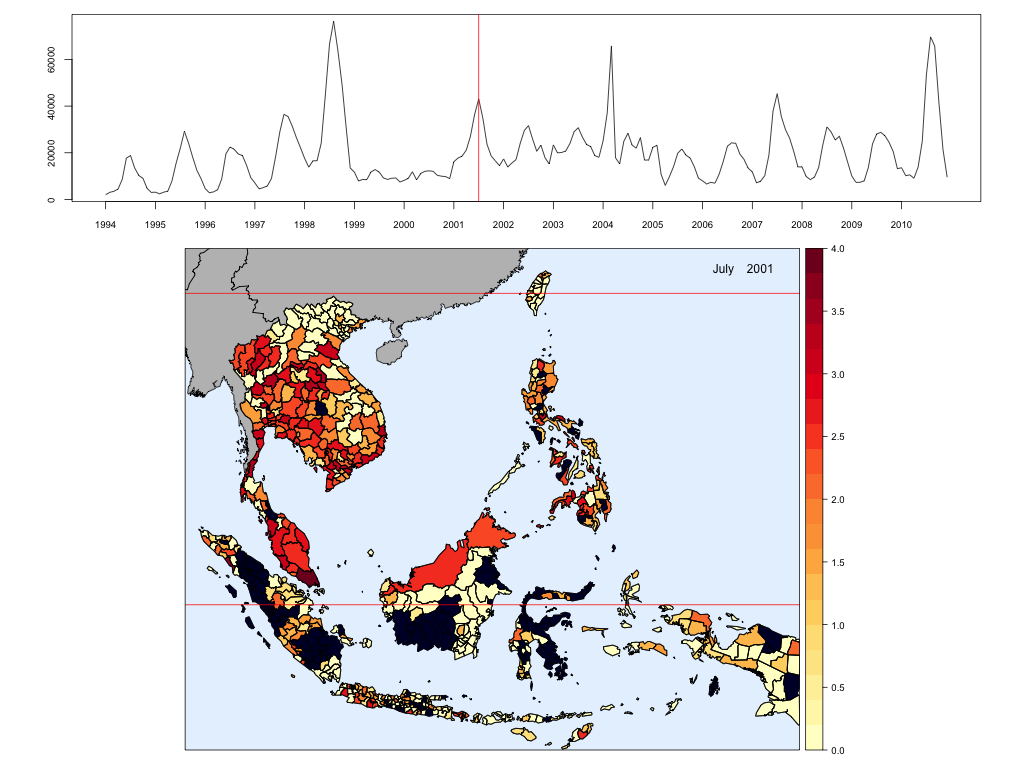
\includegraphics[width=\linewidth]{../figures/chap2/Test91.png} 
\label{fig2d}
\end{minipage}
\begin{minipage}{0.5\textwidth}
\captionof*{figure}{(e)Taux d'infection en Mars 2004  }
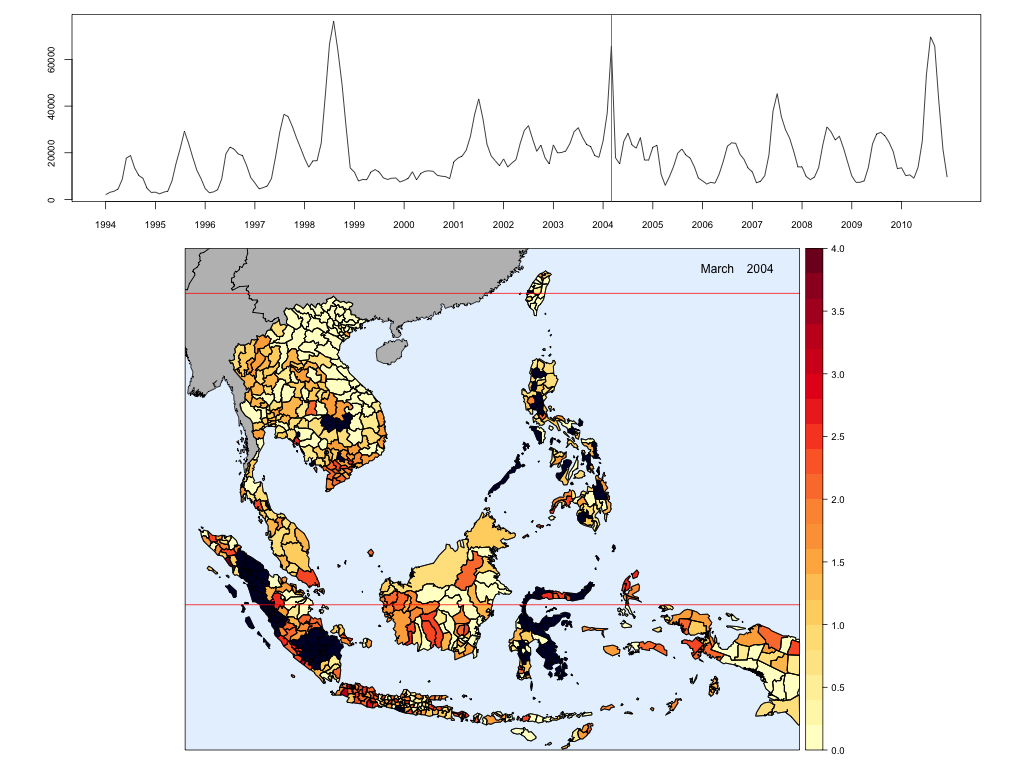
\includegraphics[width=\linewidth]{../figures/chap2/Test123.png}
\label{fig2e}
\end{minipage}\hfill
\begin{minipage}{0.5\textwidth}
\captionof*{figure}{(f)Taux d'infection en Avril 2005}  
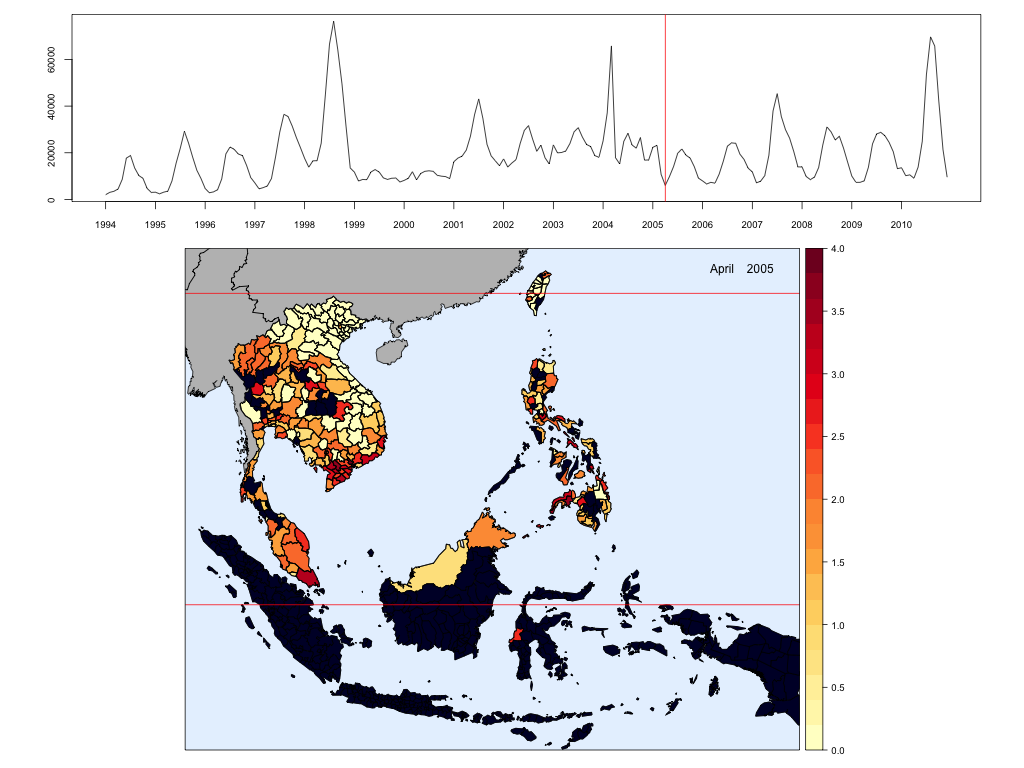
\includegraphics[width=\linewidth]{../figures/chap2/Test136.png} 
\label{fig2f}
\end{minipage}
\begin{minipage}{0.5\textwidth}
\captionof*{figure}{(g)Taux d'infection en Juillet 2007  }
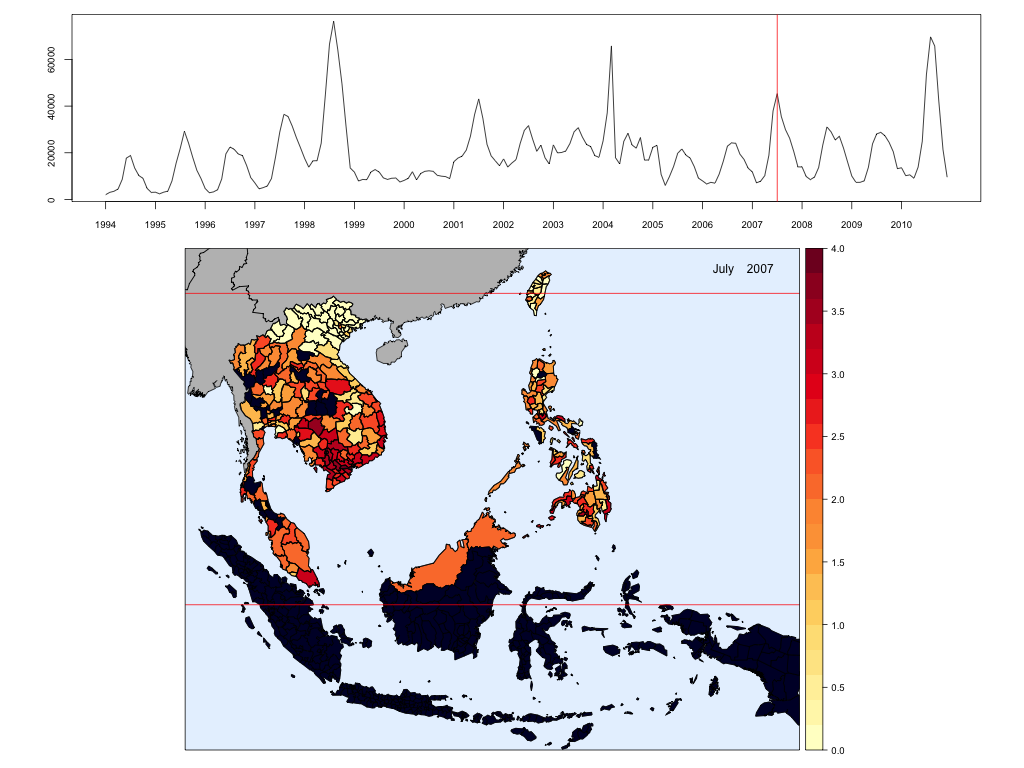
\includegraphics[width=\linewidth]{../figures/chap2/Test163.png}
\label{fig2g}
\end{minipage}\hfill
\begin{minipage}{0.5\textwidth}
\captionof*{figure}{(h)Taux d'infection en Août 2010} 
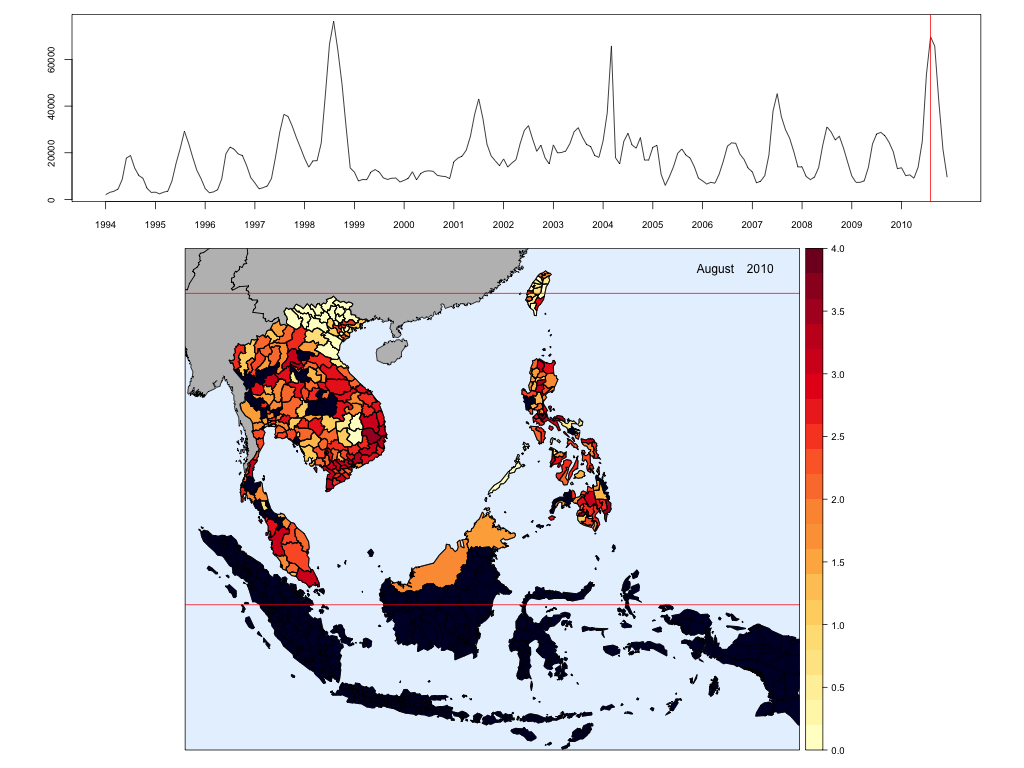
\includegraphics[width=\linewidth]{../figures/chap2/Test200.png} 
\label{fig2h}
\end{minipage}
\captionof{figure}{Le taux d'infection des provinces des pays du Sud-Est d'Asie à partir Janvier 1994 juste qu'au Décembre 2010}
\label{fig2total}
\end{center}

\section{Les donn\'ees environnementaux}
Les données mensuelle d'environnementaux sont collecté des 3 pays : Vietnam, Laos et Thaïlande. Ils contiennent les différentes facteurs climatiques aux différentes périodes. Les données environnementaux du Vietnam est été collecté par 67 station climatiques à partir Janvier 1960  au Décembre 2010. Ils comprennent les variables suivants : Température moyenne (TA), Température maximal (TX), Température minimal (TM), Pluviosité (RF), Humidité relative (RH), L'heure du soleil (SH) et Humidité absolue (AH). Ensuite, au Laos, les données environnementaux sont été collecté par 33 station climatique à partir Janvier 1998 au Décembre 2011. Ils comprennent les variables : Température maximal (TX), Température minimal (TM), Pluviosité (RF), Humidité relative maximal (RHX), Humidité relative minimal (RHM) et L'heure du soleil (SH). Tandis que les données environnementaux du Thaïlande contiennent qu'une seule variable : la pluviosité (RF) à partir Janvier 2000 juste qu'au Novembre 2011. Ces données  sont été collecté par 76 station climatique du Thaïlande. Le tableau \ref{table2.1} représente la durée, le nombre des stations et les variables du données environnementaux des 3 pays. 
\begin{table}[h]
\centering
\begin{tabular} { | c | c | c | c |}
\hline
Pays & \multicolumn {1} {p{2cm} |}{Nombre des stations climatiques} & Période du données & Variables  \\
\hline
    	      &      &                               & Température moyenne (TA)\\
	      &      &                               & Température maximal (TX) \\ 
      	      &      &                               & Température minimal (TM)\\ 
Vietnam & 67 & 01/1960 - 12/2010 & Pluviosité (RF)\\
	      &      &                               & Humidité relative (RH)\\
     	      &      &                               & L'heure du soleil (SH) \\
      	      &      &                               & Humidité absolue (AH) \\
\hline
	      &      &                               & Température maximal (TX) \\ 
      	      &      &                               & Température minimal (TM)\\ 
Laos       & 33 &  01/1998 - 12/2011& Pluviosité (RF)\\
	      &      &                               & Humidité relative maximal (RHX)\\
     	      &      &                               & Humidité relative minimal (RHM) \\
      	      &      &                               & L'heure du soleil (SH) \\
\hline
Thaïlande & 76 &  01/2000 - 11/2011& Pluviosité (RF)\\
\hline
\end{tabular}
\caption{Données climatiques des 3 pays :  Vietnam, Laos et Thaïlande} 
\label{table2.1}
\end{table}

\section{Les données du Vietnam}
\subsection {Le Vietnam}
Parmi des pays en Asie du Sud-Est, le Vietnam est un pays typique avec les condition géographie particulière où le taux d'infection est relativement élevée. Le terrain du Vietnam est étroit et horizontal qui s'étend du nord au sud. Il borde la Chine au nord, le Laos et le Cambodge à l'ouest, et la mer de l'Est à l'est. C'est pourquoi la topographie et le climat du Vietnam est divisé en 3 régions du Nord, Centre et Sud. Les données  au Vietnam sont collecté sur 64 provinces (pour la dengue) et 67 station climatiques (pour les facteurs environnementaux) et ils sont les données le plus complète durée la période. C'est la raison pour laquelle nous choisissons le Vietnam comme une échantillon pour appliquer des méthode d'analyse pour analyser la relation entre la dengue et les les facteurs environnementaux. 

\subsection {Les étapes pré-traitements des données du Vietnam}

À partir des données brutes initiales, nous avons procédé des des étapes pré-traitements pour la synchronisation de deux types de données en termes de temps et l'élimination des données vierges pour optimiser les résultats obtenus. Avant d'effectue les étapes pré-traitement, il faut d'abort modifier les données de la dengue dans quelques provinces du Vietnam à cause de la séparation et la combinaison des provinces durant 1994 - 2010. Le tableau \ref{table2.2} représente les changements des provinces dans la période 1994 - 2010. La modification des données est calculé en fonction de la taux de population des provinces après la séparation / combinaison. 
\begin{table}[h]
\centering
\begin{tabular} { | c | c | c |}
\hline
Année & Avant & Après  \\
\hline
      	 & Bac Thai & Thai Nguyen + Bac Can\\ 
      	 & Vinh Phu & Vinh Phuc + Phu Tho\\ 
      	 & Ha Bac & Bac Giang + Bac Ninh\\ 
1997 & Hai Hung & Hai Duong + Hung Yen\\ 
      	 & Ha Nam Dinh & Ha Nam + Nam Dinh\\ 
      	 & Quang Nam - Da Nang & Quang Nam + Da Nang\\ 
      	 & Song Be & Binh Duong + Binh Phuoc\\ 
      	 & Minh Hai & Ca Mau + Bac Lieu\\ 

\hline
      	 & Lai Chau & Dien Bien + Lai Chau\\ 
2004 & Hau Giang & Can Tho + Hau Giang\\ 
      	 & Dack Lak & Dak Lak + Dac Nong \\ 
\hline
2007 & Ha Noi + Ha Tay & Ha Noi\\ 
\hline
\end{tabular}
\caption{Changement des noms des provinces au Vietnam durant 1994 - 2010} 
\label{table2.2}
\end{table}
Après avoir modifier les données de la dengue à cause de la changement le nom des provinces, nous avons divisé le nombre les cas de dengue de chaque mois de chaque provinces par leurs nombre de population typique  pour obtenir le taux d'infection. Puis, nous avons effectué l'interpolation, la normalisation et le retranchement sur le taux d'infection pour obtenir des données prêtes pour les analyses. La figure 2.2 représente les étapes de pré-traitements la donnée de la dengue au Vietnam. D'après les étapes de pré-traitements, on obtenu la donnée prête à analyse dans la période de Janvier 1998 au Septembre 2010. Les données d'environnementaux du Vietnam sont aussi retranché dans le même période pour préparer à l'analyse. 
\begin{figure}[h]
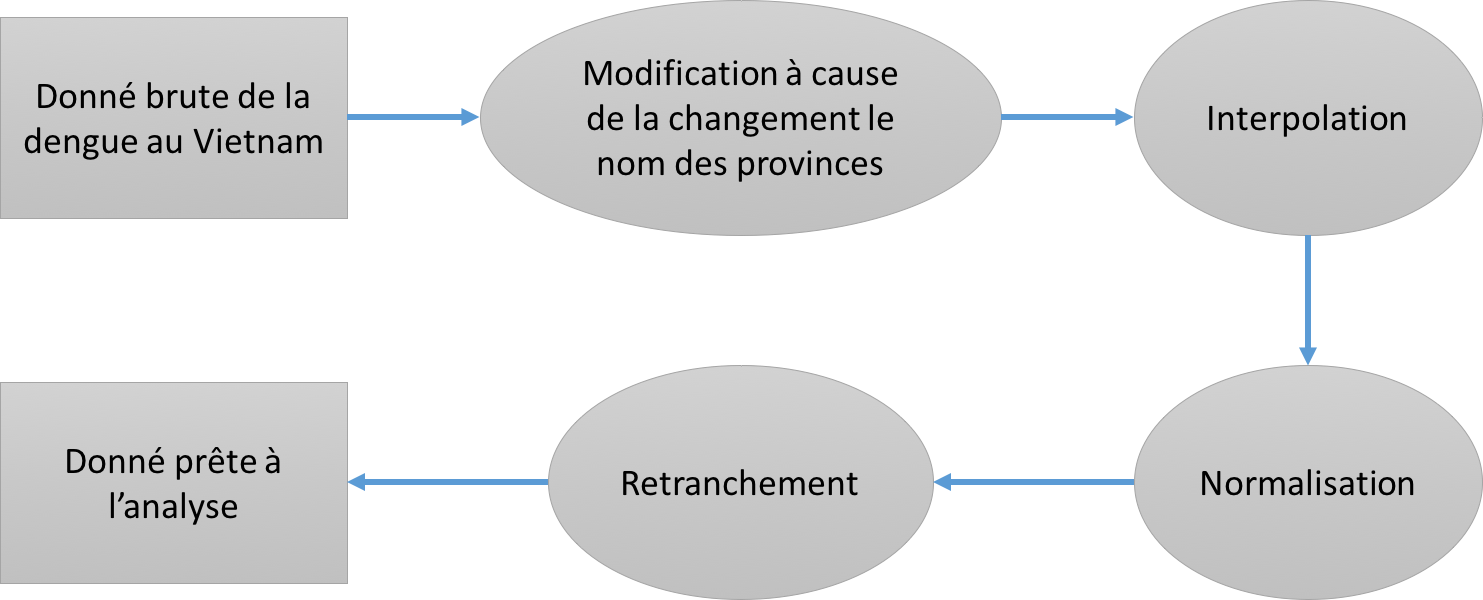
\includegraphics[width = \linewidth]{../figures/chap2/Pic2_1.png}
\caption{Les étapes de pré-traitements la donnée de la dengue au Vietnam}
\label{Pic2_1}	
\end{figure}
La figure 2.3 montre les taux d'infection de la dengue pour chaque mois, en moyenne sur les 13 années de la période d'étude et la figure 2.4 montre la même chose pour les 7 variables climatiques des 63 stations climatiques du Vietnam. Nous pouvons voir que le taux d'infection augmente fortement entre juin et novembre dans de nombreuses provinces des régions du sud et du centre-sud. Pendant cette période, les trois variables de température (maximale, minimale et moyenne) augmentent et atteignent leur nadir de façon spectaculaire en juin et juillet (milieu de la saison des pluies) avant de diminuer d'août à décembre (fin de la saison des pluies et début de saison sèche). Pendant la saison des pluies (de mai à octobre), les précipitations et l'humidité relative augmentent rapidement tandis que le nombre d'heures d'ensoleillement diminue fortement. 
Le changement apparent des facteurs climatiques et l'augmentation de l'incidence de la dengue entre juin et novembre peuvent avoir une certaine relation. Nous  appliquerons des méthodes pour analyser cette relation et représenterons dans les chapitre suivants. 
\begin{figure}[h]
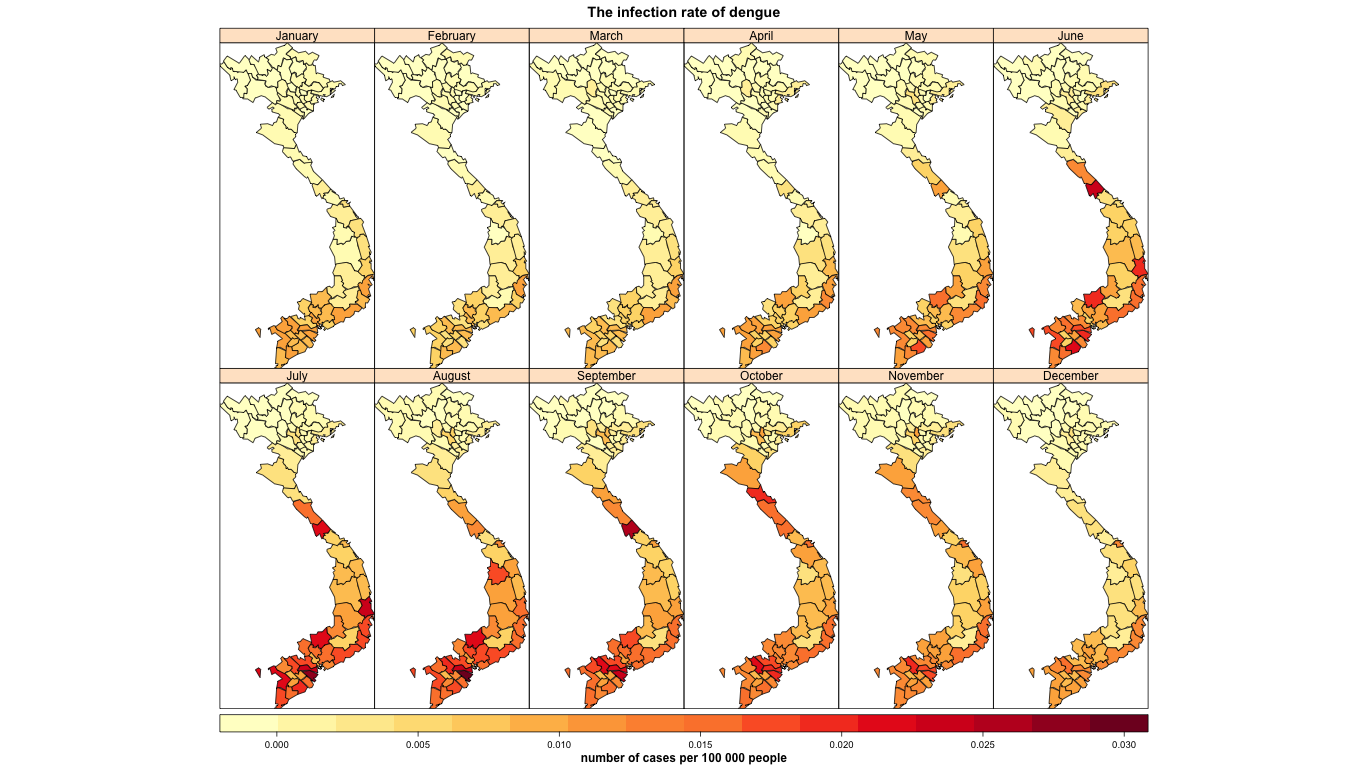
\includegraphics[width = \linewidth]{../figures/chap2/Pic2_2.png}
\caption{Incidence de la dengue par mois et province au Vietnam en moyenne sur les 13 années de janvier 1998 à septembre 2010.}
\label{Pic2_2}	
\end{figure}

\begin{figure}[h]
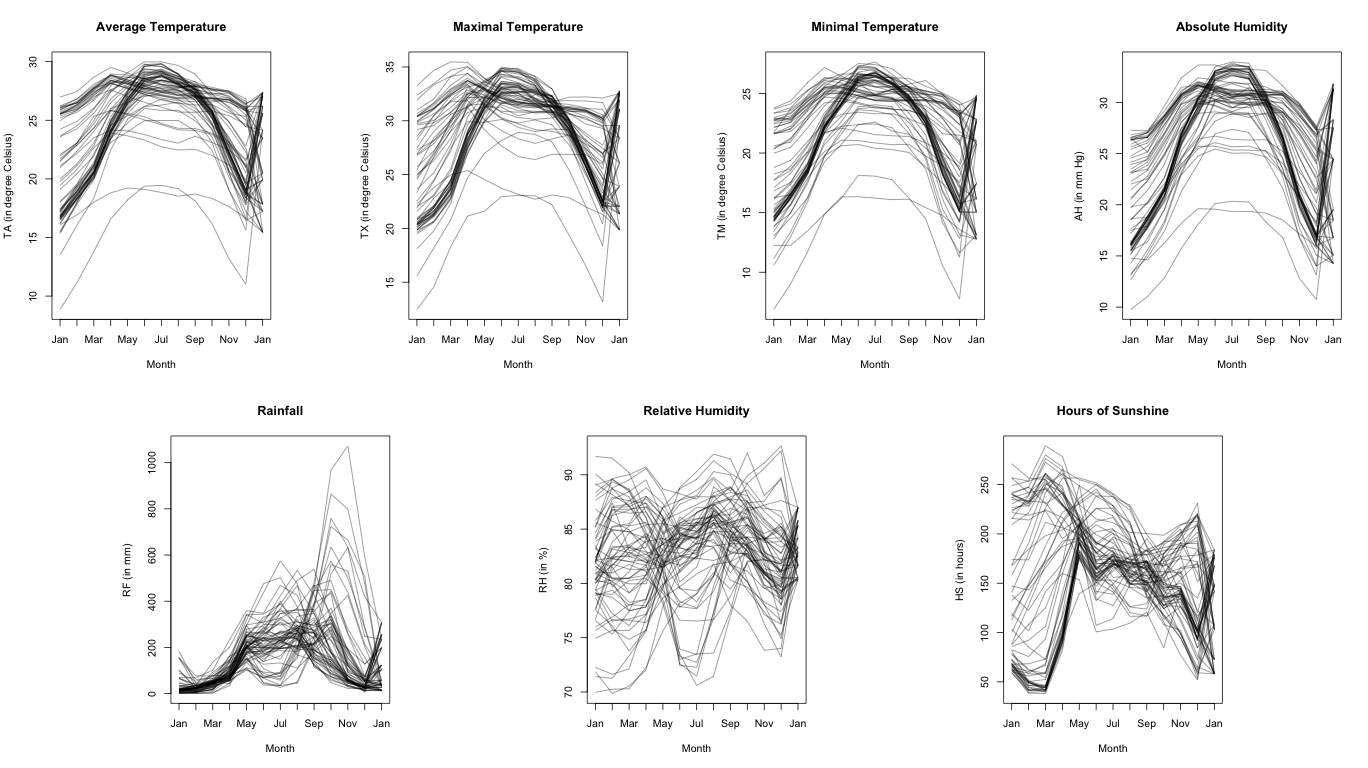
\includegraphics[width = \linewidth]{../figures/chap2/Pic2_3.png}
\caption{Variations des 7 variables climatiques par mois et stations climatiques moyennes sur les 13 années de janvier 1998 à septembre 2010.}
\label{Pic2_3}	
\end{figure}



